\documentclass{article}
\usepackage{blindtext}
\usepackage[utf8]{inputenc}
\usepackage{amsmath,bm}
\usepackage{amstext}
\usepackage{amsfonts}
\usepackage{amsmath}
\usepackage{multirow}
\usepackage{enumerate}
\usepackage{xeCJK}
\setCJKmainfont{STKaiti}
\usepackage{algorithm}
\usepackage{algorithmic}
\renewcommand{\algorithmicrequire}{ \textbf{输入:}} %Use Input in the format of Algorithm
\renewcommand{\algorithmicensure}{ \textbf{输出:}} %UseOutput in the format of Algorithm
\usepackage{graphicx}

\title{Neural Network and Applications\\Homework 1}
\author{陈轶洲 MF20330010}
\begin{document}
	\maketitle
	\numberwithin{equation}{section}
\section{试画出能够实现OR和NOT逻辑运算的感知器神经元模型,并尝试将其组合为实现XOR的感知器}
		
\hspace{1.1em} OR神经元模型:
\begin{equation}
	f(\Sigma) = y = \left\{
	\begin{aligned}
		0 \qquad\Sigma \textless 1\\
		1 \qquad\Sigma \ge 1
	\end{aligned} 
\right.
\end{equation}

\begin{figure}[H]
	\centering
	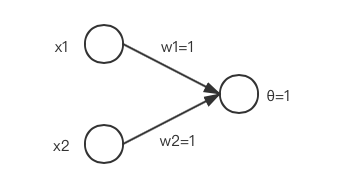
\includegraphics{OR.png}
\end{figure}


NOT神经元模型:
\begin{equation}
	f(\Sigma) = y = \left\{
	\begin{aligned}
		0 \qquad\Sigma \textless 0\\
		1 \qquad\Sigma \ge 0
	\end{aligned} 
	\right.
\end{equation}

\begin{figure}[H]
	\centering
	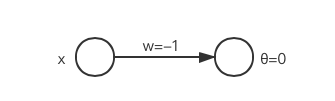
\includegraphics{NOT.png}
\end{figure}

XOR神经元模型:$\overline{(\bar{x_{1}} \cup  x_{2})}\cup  \overline{(x_{1} \cup \bar{x_{2}})}$

\begin{figure}[H]
	\centering
	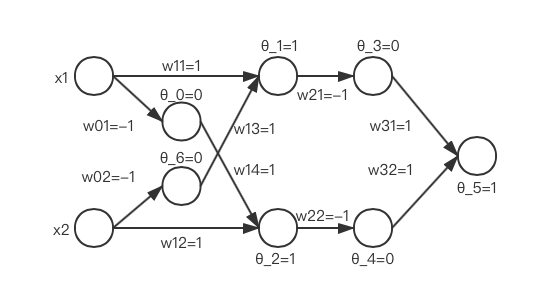
\includegraphics[scale=0.8]{XOR.png}
\end{figure}



\newpage
\section{利用最小二乘法求解下列x,y关系的线性回归方程,并利用单神经元表示
}
	\begin{table}[h]
	\centering
	\label{tab:my_label}
	\begin{tabular}{|c|c|c|c|c|c|c|c|c|c|c|}
		\hline
		x & 24 & 15 & 23 & 19 & 16& 11& 20 &16 &17 &13\\
		\hline
		y & 92 & 79& 97& 89 & 64& 47& 83& 68& 71& 59\\
		\hline
	\end{tabular}
	
\end{table}
使用单元线性回归中的最小二乘法,容易求得
\begin{equation}
	\begin{aligned}
		\bar{x} &= 17.4 \qquad \bar{y} = 74.9\\
		\sum_{i=1}^{10}{x_{i}y_{i}}&=13578 \qquad \sum_{i-1}^{10}{x_{i}^{2}}=3182
	\end{aligned}
\end{equation}
结合公式可知
\begin{equation}
	\begin{aligned}
		w=\dfrac{\sum_{i=1}^{10}{x_{i}y_{i}}- n\bar{x}\bar{y}}{\sum_{i-1}^{10}{x_{i}^{2}}-n\bar{x}^{2}}=\dfrac{13578-13032.6}{3182 - 3027.6}\approx 3.53\\
		b=\bar{y}-w\bar{x}=74.9 - 3.53\times 17.4=13.44
	\end{aligned}
\end{equation}
单神经元表示为
\begin{figure}[H]
	\centering
	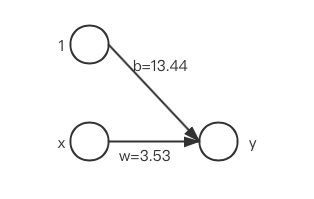
\includegraphics{LG.png}
\end{figure}



\end{document}
